\section{Introduction}\label{Section_introduction}

\begin{wrapfigure}{r}{9cm}
	\centering
	\vspace{-0.3cm}
	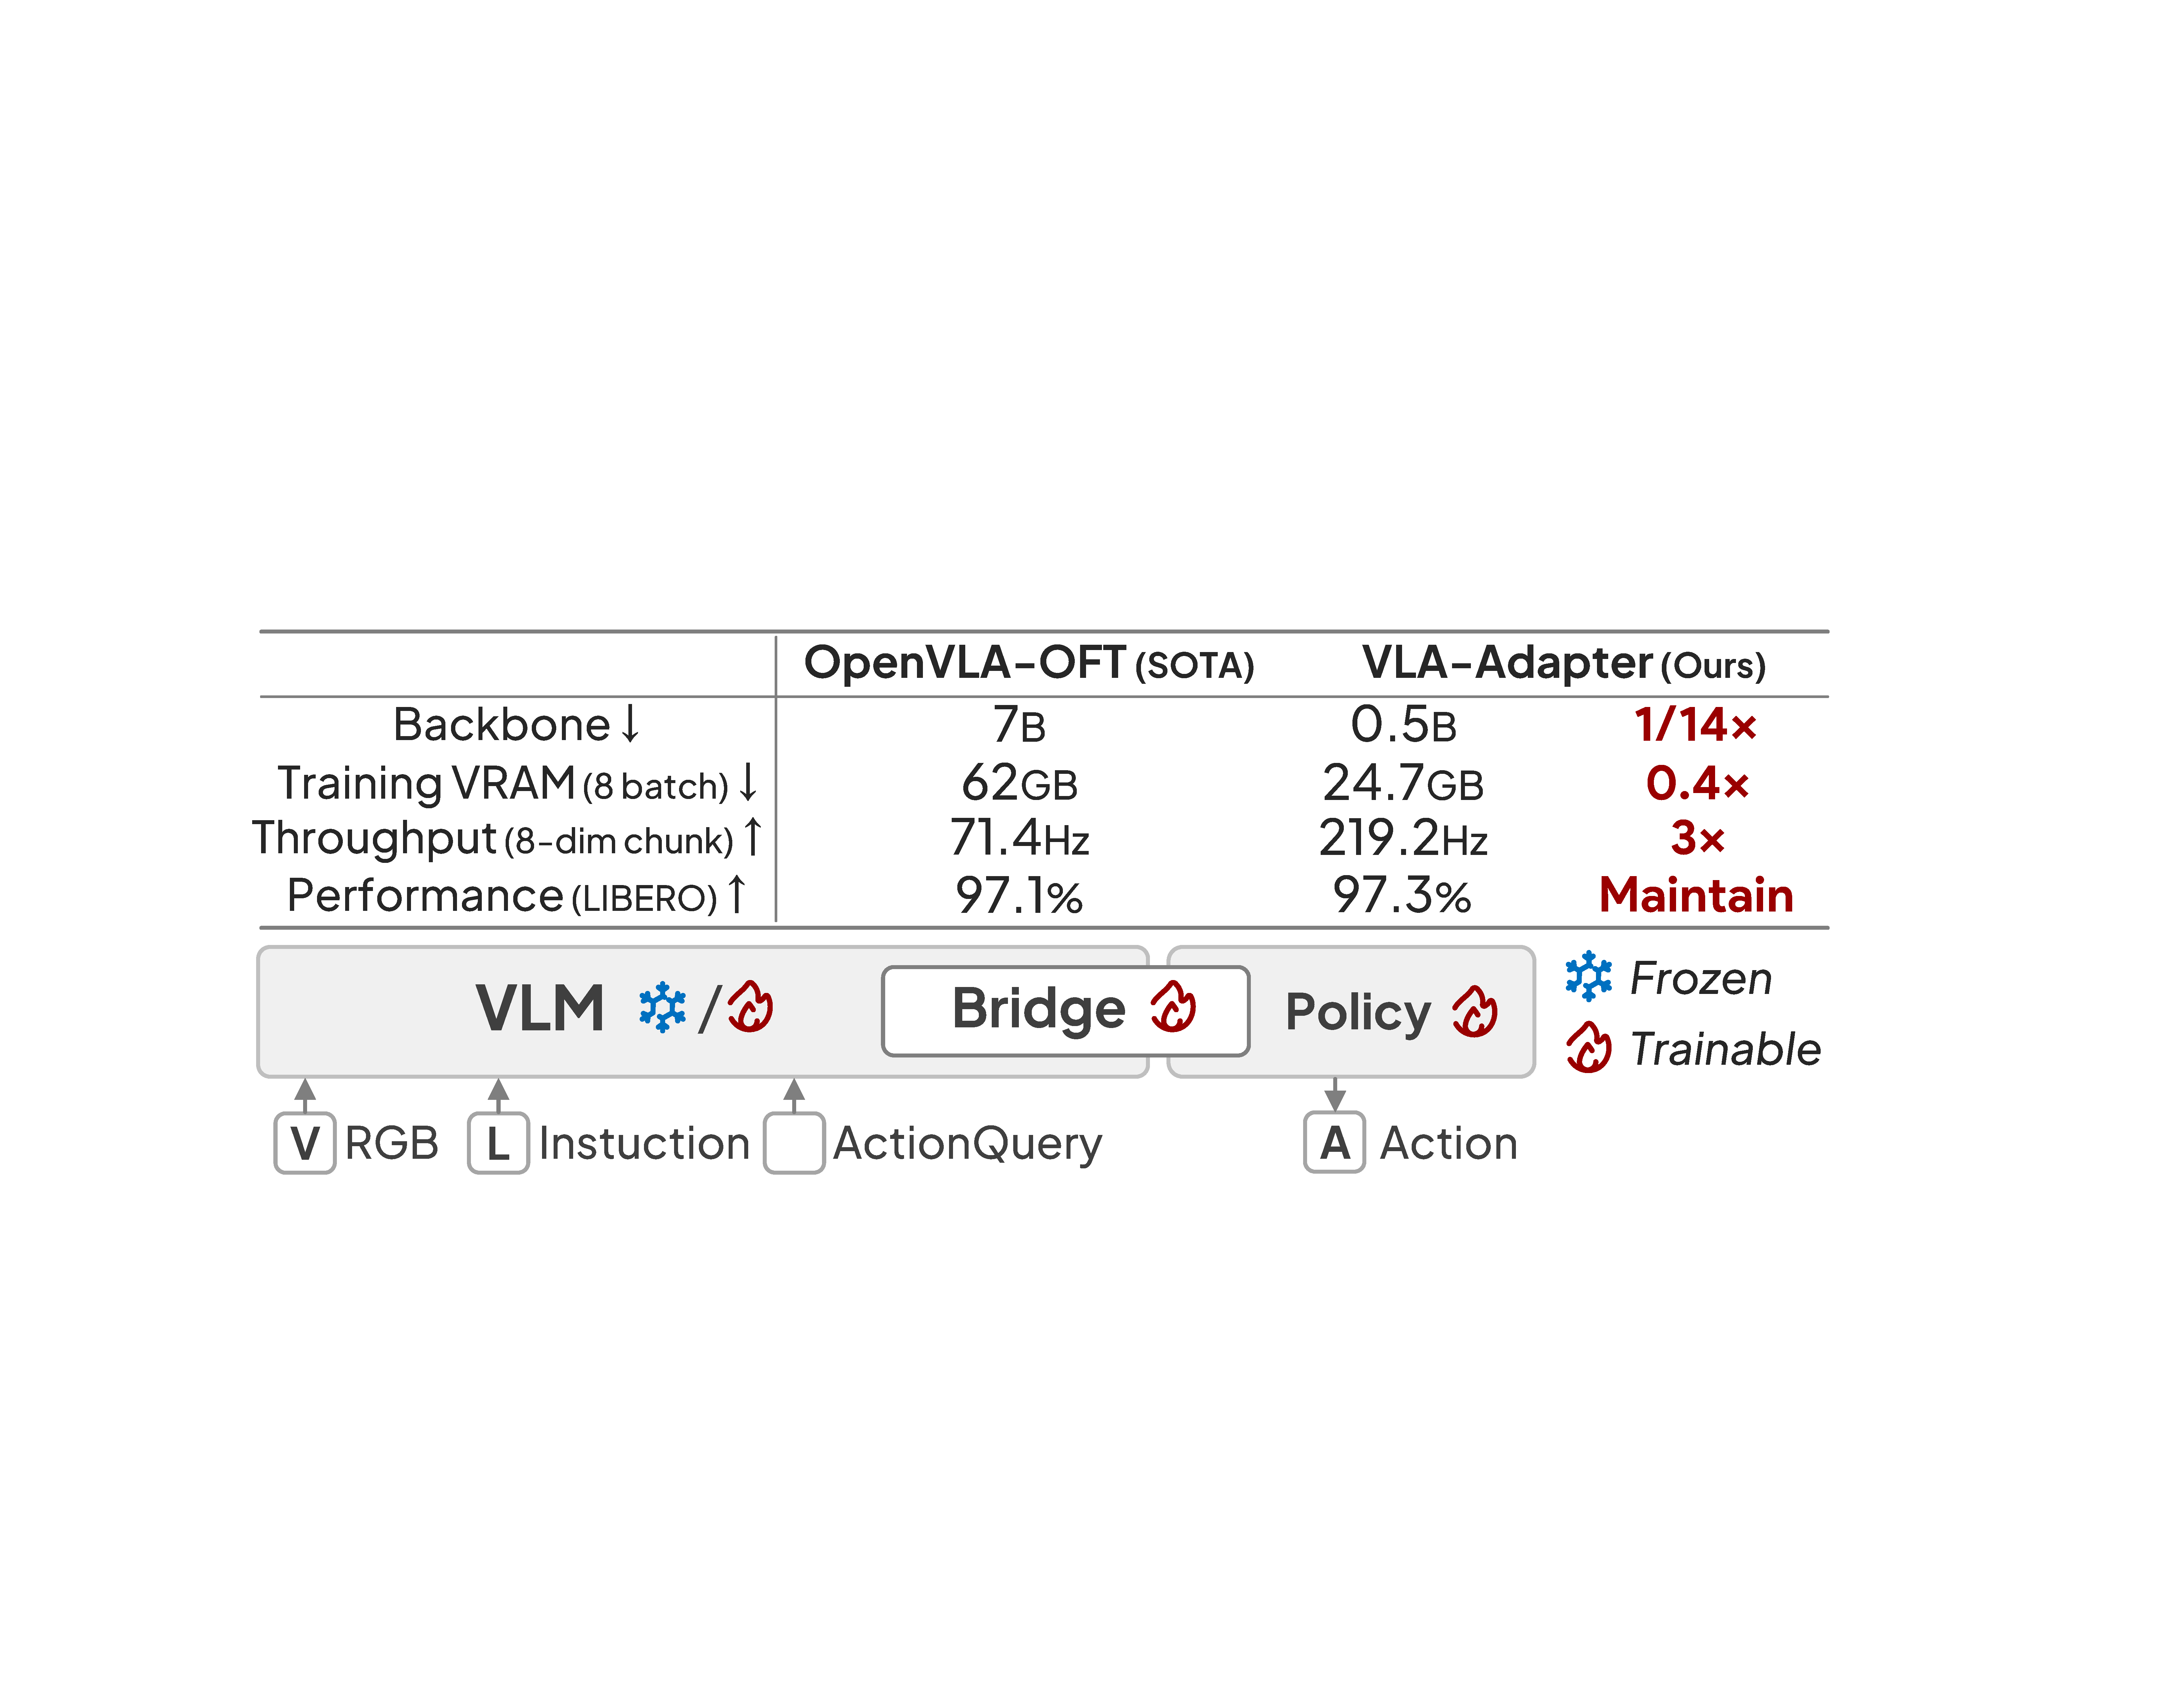
\includegraphics[width=0.6\textwidth]{Figures/Teaser.pdf}
	\vspace{-0.1cm}
	\caption{Characteristics of VLA-Adapter. ``$\downarrow$" is that smaller values are better, and vice versa. Our paradigm can effectively obtain the SOTA-level VLA model using a tiny-scale backbone.}\label{Figure_teaser}
	\vspace{-0.25cm}
\end{wrapfigure}

In the past two years, with significant breakthroughs in multimodal LLMs \citep{Prismatic-2024, PaliGemma-2024, LLaVA-2023, Eagle-2-2025}, developing robot systems with general perception, understanding, and behavior capabilities has become a key research direction in artificial intelligence. In particular, the emergence of the Vision-Language-Action (VLA) model offers a new solution for enabling robot operations driven by instructions \citep{OpenVLA-2024, OpenHelix-2025, OpenVLA-OFT-2025, PDVLA-2025, WorldVLA-2025, DreamVLA-2025, MemoryVLA-2025}. Research on VLA primarily focuses on extracting multimodal information and aligning it with the action space to generate the high-quality actions \citep{Octo-2024, RDT-2025, FlowVLA-2025, LongVLA-2025}.

Current VLA models typically require large-scale embodied data (e.g., Open X-Embodiment \citep{OpenX-2024} and DROID \citep{DROID-2024}) to pre-train Multimodal Large Language Models (MLLMs) (Especially, VLMs) for task adaptability \citep{GR-2-2024}, which is then passed to the designed Policy network \citep{RoboDual-2024, RoboFlamingo-2024} to decode or generate actions for handling the tasks in the diverse environments \citep{LIBERO-2023, CALVIN-2022}. 

However, when confronted with high-dimensional control environments, VLA models still face several bottlenecks, including reliance on large-scale VLMs, slow fine-tuning speed, high GPU memory (VRAM) consumption, and low inference efficiency (throughput), as shown in Figure \ref{Figure_teaser}. To this end, it is necessary to explore the most essential but rarely discussed question in the VLA field: \textbf{\textit{How to bridge the gap of VL (vision-language representations) to A (action) more effectively?}}

To answer this question, we propose VLA-Adapter, a novel bridging paradigm for VLA. We systematically explore how different conditions influence action generation and give some key findings for VLA design. On this basis, we built a Policy network with Bridge Attention to autonomously inject the optimal condition into the action space. Experiments show that VLA-Adapter has superior performance, high inference efficiency, and fast throughput with a tiny-scale backbone. It significantly lowers the barrier to VLA deployment. The main contributions are summarized as follows.

\begin{itemize}
	\item To our knowledge, this work is the first systematic analysis of bridging paradigms' effects on action generation. And we also give some key findings of the VLA model design.
	\item VLA-Adapter transfers the sufficient multimodal information to the proposed Policy Network for action generation, effectively bridging the modality gap from VL to A. 
	\item Rich experiments show that VLA-Adapter has a higher success rate, smaller scale, lower tuning cost, and faster inference in diverse simulated and real-world robotic tasks.
\end{itemize}